\section{Introduction}

\subsection{Motivation}


\begin{frame}{Motivation}
  \begin{itemize}
    \item Rise of World Wide Web led to better communication
    \item Place to meet and exchange information easily
    \item Researches took this opportunity to transform Communities of Practice into online Communities of Practice (CoPs)
          \begin{itemize}
            \item World-wide collaboration
          \end{itemize}
          %researchers in particular from all over the world can collaborate more easily 
          %what Cops are will be discussed in more detail later.
  \end{itemize}

\end{frame}

\begin{frame}{Motivation}
  \begin{itemize}
    \item Success of CoP relies on success factors, which are changing over time
    \item It is difficult to measure and evaluate them
          \begin{itemize}
            \item Domain-specific success factors
            \item Time consuming
            \item Require data-management experts %which especially small CoPs lack
          \end{itemize}
    \item Success modeling systems automate success evaluation
  \end{itemize}
\end{frame}

\begin{frame}{Motivation}
  %this is why some continuous success modeling systems have been developed
  %however, the problem is that
  \begin{columns}
    \begin{column}[]{0.4\textwidth}

      Traditional success modeling systems
      \begin{itemize}
        \item Complicated, as they require technical know-how
        \item Not optimized for collaboration
        \item Do not take mobility into consideration
      \end{itemize}

    \end{column}
    \begin{column}[]{0.6\textwidth}
      Social Networks and chat platforms are used for information exchange
      \begin{itemize}
        \item Familiar and intuitive
        \item Real-time collaboration
        \item Optimized for mobile devices
      \end{itemize}
      %This shows how chat platforms could adress the aforementionted issues
    \end{column}
  \end{columns}

\end{frame}


\subsection{Thesis Goals}

\begin{frame}{Thesis Goals}
  \begin{itemize}
    \item Design a chatbot for success modeling and visualizations
          inside Community Information Systems (CIS)
    \item Find out how the bot affects collaboration and success awareness of the commmunity %in contrast to traditional web frontends
  \end{itemize}
\end{frame}

\section{State of the Art}

\subsection{Social Bots}
\begin{frame}{Social Bots and Chatbots}
  \begin{block}{Definition}
    ``A social bot is a computer algorithm that automatically produces content and interacts with humans on social media, \dots'' \cite{FVD*16b}
  \end{block}
\end{frame}
\begin{frame}{Social Bots and Chatbots}
  \begin{block}{Definition}
    ``A social bot is a computer algorithm that automatically produces content and interacts with humans on social media, \dots'' \cite{FVD*16b}
  \end{block}
  \begin{itemize}
    \item Can be used for automation  %e.g. Alexa Smart Home, Shopping lists Reminders
    \item Users interact with Bots by voice or chat %in the case of chat: Chatbots
    \item Provide better user experience, as they are more intuitive to use
  \end{itemize}
\end{frame}

\subsection{Succes in Communities of Practice}
\begin{frame}{Communities of Practice}
  \begin{block}{Definition}
    ``Communities of practice are groups of people who share a concern or a
    passion for something they do and learn how to do it better as they interact regularly.'' \cite{Weng98}
  \end{block}
\end{frame}

\begin{frame}{Communities of Practice}
  \begin{block}{Definition}
    ``Communities of practice are groups of people who share a concern or a
    passion for something they do and learn how to do it better as they interact regularly.'' \cite{Weng98}
  \end{block}
  \begin{itemize}
    \item CoPs are  diverse communities
    \item Informal structures with permeable boundaries \cite{RKJa15}
    \item CoPs contain sub-commmunities which can be overlapping
  \end{itemize}
\end{frame}


\begin{frame}{Members of a Communitiy of Practice}
  \begin{itemize}
    \item Have various roles
          \begin{itemize}
            \item Researchers
            \item Professionals
            \item Students
            \item Hobbyists
          \end{itemize} %DBIS and ACIS as an example????
    \item Have different degrees of
          \begin{itemize}
            \item Knowledge %Researchers > students
            \item Interest %Professionals > Hobbyists
            \item Contribution
                  \begin{itemize}
                    \item Core Members %do most of the contribution 
                    \item Lurkers %only consume but almost no contribution
                          %study on open Source found that for random projects 22percent contribute. For the top 500 projects: ~90percent don't contribute -> 1% (90-9-1) rule
                  \end{itemize}
          \end{itemize}
    \item Do not have to belong to the same organization
    \item Share their work through social interaction e.g. online Social Networks %in this case we also talk about an online CoP

  \end{itemize}
\end{frame}


\begin{frame}{Measurement of Success}
  \begin{columns}
    \begin{column}[]{0.3\textwidth}
      \begin{itemize}
        \item Communities of Practice need to be aware of their success
              \begin{itemize}
                \item Improve their work
                \item Adjust to current trends
              \end{itemize}
              %Success seems to be a very abstract metric so in order to measure it we build a success model
        \item Measurement of Success through a \emph{Success Model}
        \item Success model distinct for each community

      \end{itemize}
    \end{column}
    \begin{column}[]{0.7\textwidth}
      \begin{figure}
        \centering
        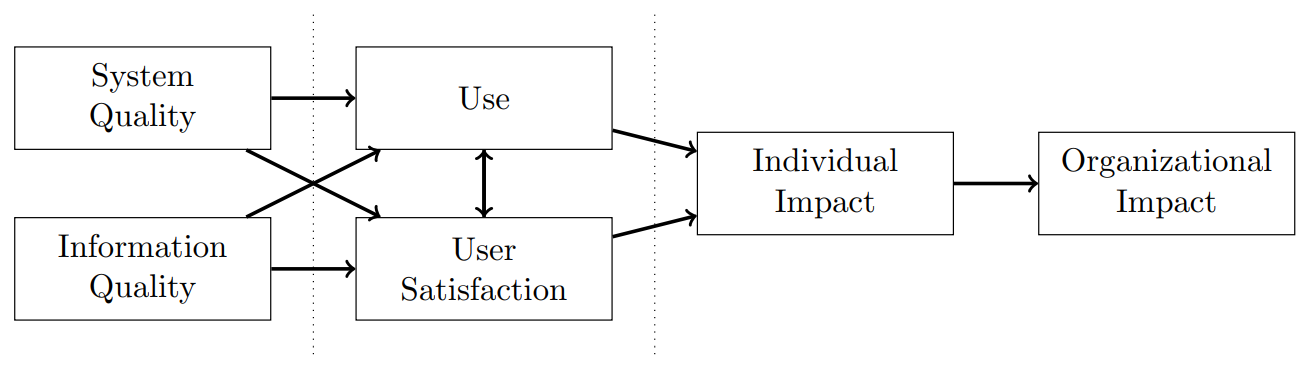
\includegraphics[width=\textwidth]{related_work/deloneMclean.png}
        \caption{Community Information Systems Success Model by DeLone and McLean \cite{DeMc92}}
        %13!!!!
      \end{figure}
    \end{column}
  \end{columns}
\end{frame}



\begin{frame}{MobSOS}

  \begin{itemize}
    \item MobSOS success model is based on the success model of DeLone and McLean
    \item Core Component of las2peer
    \item Monitors las2peer services
    \item MobSOS Continuous Community Analytics extends MobSOS
          \begin{itemize}
            \item Provides visualizations of MobSOS data
            \item Ability to dynamically add databases and Mediabases
          \end{itemize}
  \end{itemize}
  %The MobSOS cca also allows the addition of Mediabases, which can be used to gather data produced outside the las2peer environment
\end{frame}

\begin{frame}{Mediabase}
  \begin{columns}

    \begin{column}[]{0.4\textwidth}
      \begin{itemize}
        \item Proposed to handle Web 2.0 data in a more effective way
        \item Mediabase includes
              \begin{itemize}
                \item Backend database (DB2 or MySQL)
                \item Crawler scripts
                \item Monitoring processes
                \item Frontend for user interactions
              \end{itemize}
      \end{itemize}
    \end{column}

    \begin{column}[]{0.6\textwidth}
      \begin{figure}[h]
        \centering
        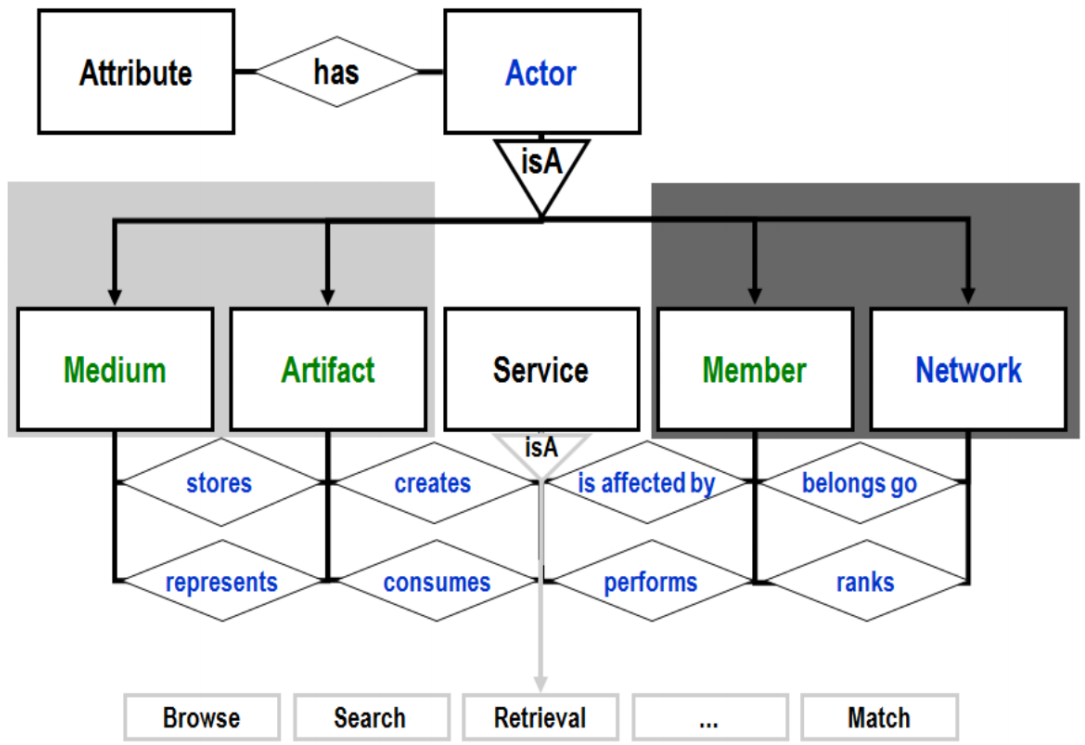
\includegraphics[height=0.8\textheight]{related_work/mediabase.png}
        \caption{Mediabase Overview \cite{Klam10e}}
      \end{figure}
    \end{column}

  \end{columns}
\end{frame}



\section{Concept}
\subsection{Use Case}
\begin{frame}{Mensa Communities}
  \begin{itemize}
    \item Community of people frequently visiting the mensa
    \item Community consists of students and university employees
    \item Similar to the concept of Community of Practice %share a concern: food at the canteen. And Interact regularly: Students argumenting on which mensa is the best?? Freqwuent visits to mensa
    \item Different community levels:
          \begin{itemize}
            \item Top level: all mensa frequenteers in Germany
            \item Intermediate level: all mensa frequenteers for a University
            \item Low level: individual circle of friends, which frequent the canteen together %Members can belong to different circles of friends->overlapping
          \end{itemize}
  \end{itemize}
\end{frame}



% \begin{frame}{Mensa Bot}
%   For this community a chatbot is designed, which can be used to
%   \begin{itemize}
%     \item Get the menu for a canteen
%     \item Rate meals
%     \item Query success visualizations for meals, canteens and other success metrics, which can be designed by the community
%   \end{itemize}
%   The chatbot is deployed with Slack.
% \end{frame}

\begin{frame}{Use case diagram for the Chatbot}
  \begin{figure}
    \centering
    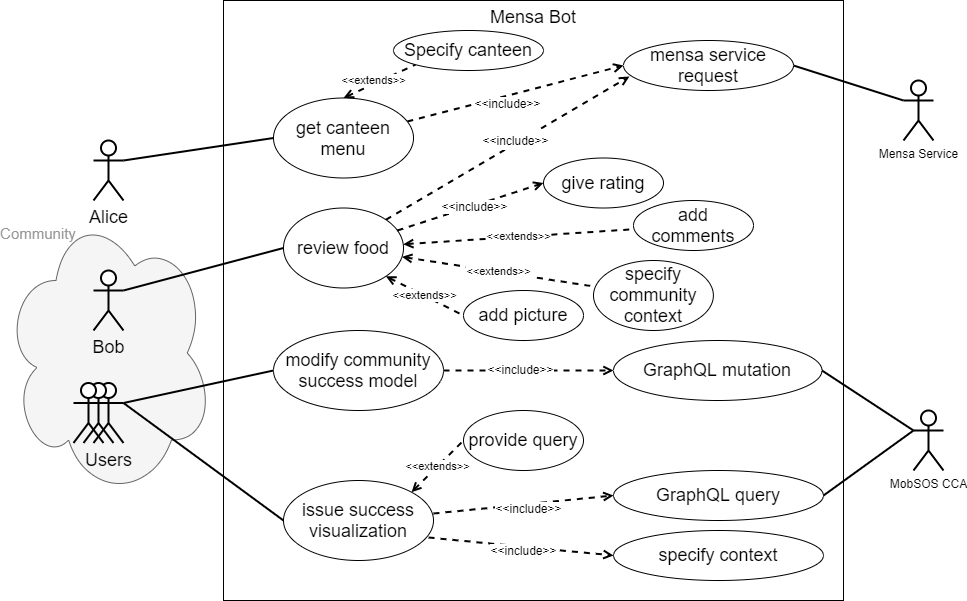
\includegraphics[height=0.85\textheight]{concept/usecase.png}

  \end{figure}
\end{frame}

\subsection{System overview}

\begin{frame}{System overview}
  \begin{figure}
    \centering
    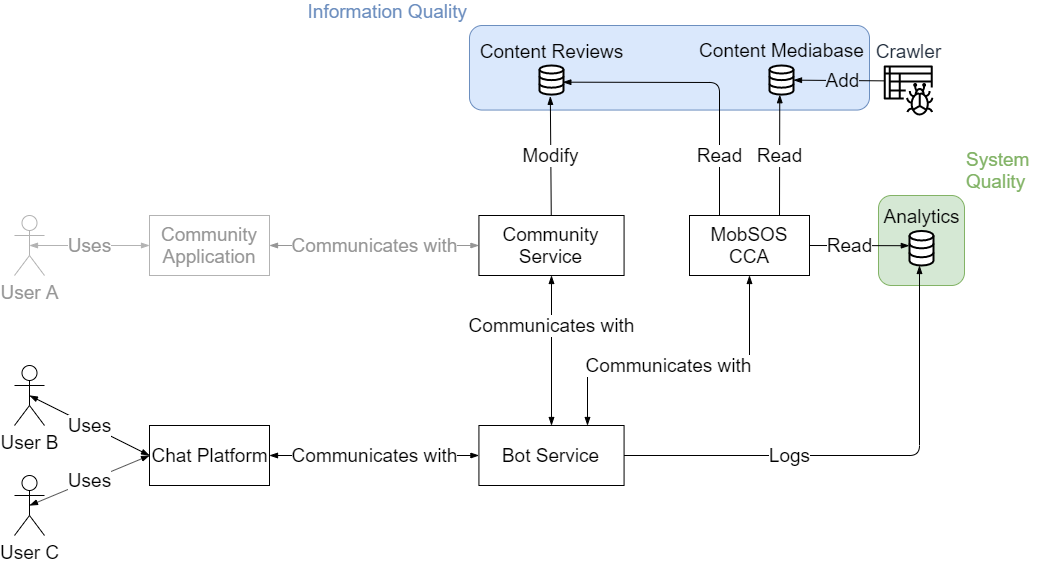
\includegraphics[height=0.85\textheight]{realization/Component_Diagramm.png}

    \label{fig:sytsemOverview}
  \end{figure}
\end{frame}

\section{Realization}

\begin{frame}\begin{columns}
    \begin{column}[]{0.7\textwidth}
      \begin{figure}
        \centering
        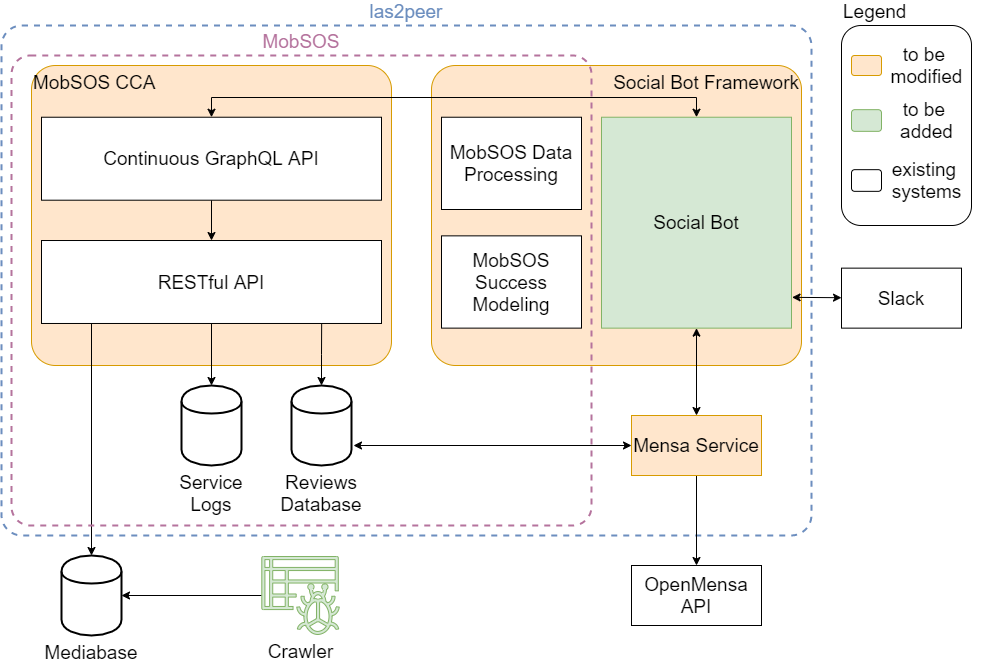
\includegraphics[height=0.9\textheight]{realization/components_overview.png}
        \caption{Overview of the different components}
        \label{fig:componentsOverview}
      \end{figure}
    \end{column}
    \begin{column}[]{0.3\textwidth}
      Technologies:
      \begin{itemize}
        \item las2peer
        \item MobSOS
              \begin{itemize}
                \item MobSOS CCA
                \item MobSOS Data Processing
                \item MobSOS Success Modeling
              \end{itemize}
        \item Mediabase
              \begin{itemize}
                \item Javascript Crawler for Twitter
              \end{itemize}
        \item Social Bot Framework
        \item Mensa Service
        \item Chat Platforms
              \begin{itemize}
                \item Slack
                \item Telegram
                \item Rocket Chat
              \end{itemize}
      \end{itemize}
    \end{column}
  \end{columns}

\end{frame}

\begin{frame}{Use of Community Service in Private Chat}
  \begin{columns}
    \begin{column}[]{0.6\textwidth}
      \begin{figure}
        \centering
        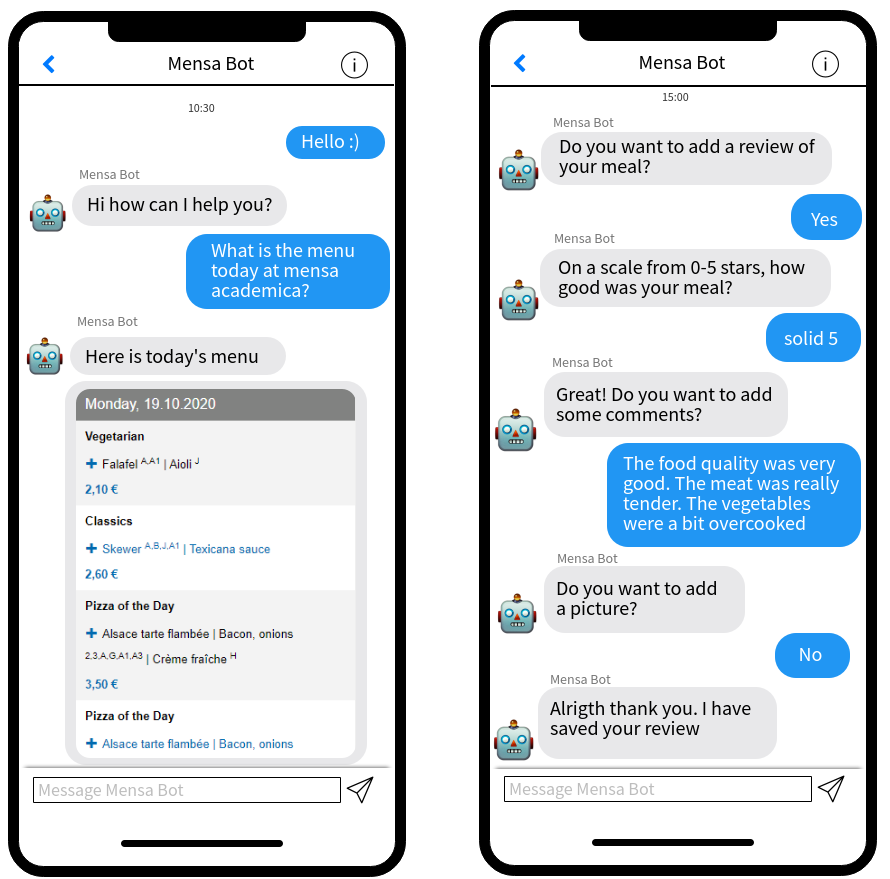
\includegraphics[height=0.85\textheight]{realization/chat_mockup.png}

      \end{figure}
    \end{column}
    \begin{column}[]{0.4\textwidth}
      \begin{enumerate}
        \item Menu request intent recognized
              \begin{itemize}
                \item Mensa service GET request
              \end{itemize}
        \item Mensa service response
        \item Mensa service POST request
      \end{enumerate}
    \end{column}
  \end{columns}

\end{frame}

\begin{frame}{Visualization Request in Group Chat}
  \begin{columns}
    \begin{column}[]{0.5\textwidth}
      \begin{figure}
        \centering
        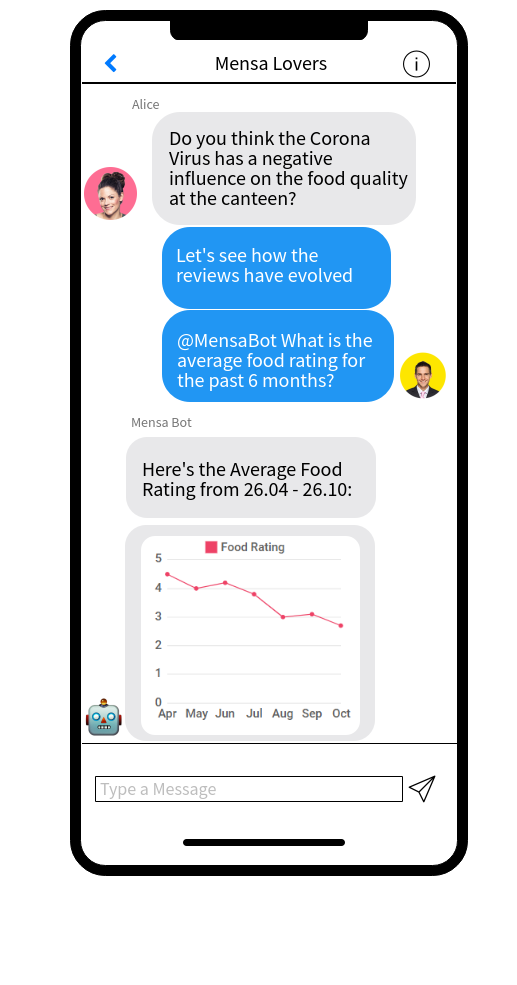
\includegraphics[height=0.85\textheight]{realization/visual_req.png}
      \end{figure}
    \end{column}
    \begin{column}[]{0.5\textwidth}
      \begin{enumerate}
        \item Average food Rating request intent recognized
              \begin{itemize}
                \item MobSOS CCA request based on template
              \end{itemize}
        \item MobSOS CCA response
      \end{enumerate}
    \end{column}
  \end{columns}
\end{frame}

\section{Evaluation}

% \begin{frame}{Thesis questions -hier stehn todos und keine thesis goals}
%   \begin{itemize}
%     \item Does the use of chatbots increase the success awareness of the community?
%     \item Does it increase collaboration between members?
%     \item Does it improve the user experience in terms of mobility?
%   \end{itemize}
% \end{frame}

\begin{frame}{Data Collection}
  \begin{itemize}
    \item Research question: What is the impact of the chatbot on the community
          \begin{itemize}
            \item Collaboration
            \item Success awareness
            \item Mobility
          \end{itemize}
    \item Chatbot will be deployed to various platforms for collecting reviews
    \item Crawler script collects reviews from webpages
  \end{itemize}
\end{frame}

\begin{frame}{Overview}
  \begin{itemize}
    \item Find mensa commmunity
    \item \begin{itemize}
            \item people which frequently visit the canteen
          \end{itemize}
    \item Participants are part of the mensa commmunity
    \item Evaluation will be done on two phases:
          \begin{itemize}
            \item  Community Service Phase
            \item Success modeling phase
          \end{itemize}
  \end{itemize}
\end{frame}


\begin{frame}{Community Service Phase}
  \begin{itemize}
    \item Evaluate the usability of the bot for getting menu and making reviews
    \item Volonteers will be acting as community members
    \item Members will join a new Mensa Slack group
    \item The chatbot is included in a group channel
          \begin{itemize}
            \item can be used to query menu
          \end{itemize}
    \item Members are asked to make a food review by Direct Message with the bot
    \item Hand out questionnaire covering usability of the bot
    \item Feedback is included into the success model
  \end{itemize}
\end{frame}

\begin{frame}{Success Modeling Phase}
  \begin{itemize}
    \item Evaluate the collaboration aspect of the bot
    \item Preferably same volonteers as first phase %maybe some new features were added in the first phase which they can now try out... See their impact on the community
    \item Divide into groups of 2-3 students
          \begin{itemize}
            \item make visualization requests
            \item update the success model
          \end{itemize}
    \item Hand out questionnaire covering collaboration and success awareness
  \end{itemize}
\end{frame}

\section{Project Plan}

\begin{frame}
  \begin{figure}
    \centering
    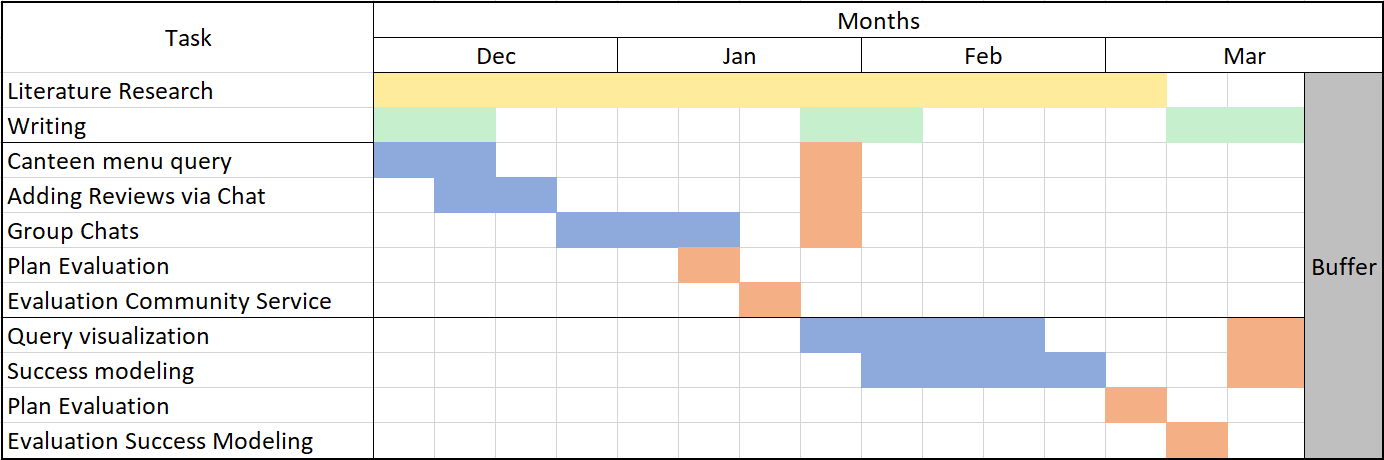
\includegraphics[width=0.89\textwidth]{project_plan/projectplan.png}

    \label{fig:visualReq}
  \end{figure}
\end{frame}